\documentclass[aspectratio=169,12pt]{beamer}

% ---------------------------------------------------------------------------
% Mid-Semester Evaluation: Reliability-Weighted Ensembling for Cross-Domain
% LLM Session Recommendation
%
% 25 frames (including title). Every frame is sized to fit at normal font --
% content was split across frames rather than shrunk to fit.
%
% CHANGES IN THIS VERSION:
%   - Fixed fatal "lonely \item" error on the title frame
%   - RWRA now expanded on first use (pipeline frame + Step 1 frame)
%   - NEW frame: output protocol and strict parsing
%   - NEW frame: per-session drift score
%   - "Results" frame retitled (n=5 is a pilot, not a result)
%   - Fixed broken "(below)" cross-reference
%   - Fixed punctuation on the self-consistency bullet
% ---------------------------------------------------------------------------

\usetheme{Boadilla}
\usecolortheme{dove}
\usefonttheme{professionalfonts}
\setbeamertemplate{navigation symbols}{}

\usepackage[T1]{fontenc}
\usepackage[utf8]{inputenc}
\usepackage{amsmath,amssymb}
\usepackage{array,booktabs,tabularx,multirow}
\usepackage{graphicx}
\usepackage{hyperref}
\usepackage{ragged2e}
\usepackage{xcolor}
\usepackage{tikz}
\usetikzlibrary{arrows.meta,calc,fit,positioning,shapes.geometric}

% Palette
\definecolor{DeepBlue}{HTML}{143D59}
\definecolor{Teal}{HTML}{087E8B}
\definecolor{Orange}{HTML}{F28F3B}
\definecolor{SoftBlue}{HTML}{EAF2F8}
\definecolor{SoftTeal}{HTML}{E8F6F3}
\definecolor{SoftOrange}{HTML}{FFF3E8}
\definecolor{Ink}{HTML}{263238}
\definecolor{Muted}{HTML}{607D8B}
\definecolor{LightGray}{HTML}{D9E2E8}

\setbeamercolor{structure}{fg=DeepBlue}
\setbeamercolor{normal text}{fg=Ink,bg=white}
\setbeamercolor{frametitle}{fg=DeepBlue,bg=SoftBlue}
\setbeamercolor{title}{fg=DeepBlue}
\setbeamercolor{subtitle}{fg=Muted}
\setbeamercolor{block title}{fg=white,bg=DeepBlue}
\setbeamercolor{block body}{fg=Ink,bg=SoftBlue}
\setbeamercolor{block title alerted}{fg=white,bg=Orange}
\setbeamercolor{block body alerted}{fg=Ink,bg=SoftOrange}
\setbeamercolor{block title example}{fg=white,bg=Teal}
\setbeamercolor{block body example}{fg=Ink,bg=SoftTeal}
\setbeamerfont{frametitle}{series=\bfseries,size=\Large}
\setbeamerfont{title}{series=\bfseries,size=\Huge}
\setbeamerfont{subtitle}{size=\large}

\setbeamertemplate{footline}{%
  \leavevmode%
  \hbox{%
    \begin{beamercolorbox}[wd=.82\paperwidth,ht=2.6ex,dp=1.1ex,leftskip=1em]{author in head/foot}%
      \usebeamerfont{author in head/foot}\insertshorttitle
    \end{beamercolorbox}%
    \begin{beamercolorbox}[wd=.18\paperwidth,ht=2.6ex,dp=1.1ex,center]{date in head/foot}%
      \usebeamerfont{date in head/foot}\insertframenumber/\inserttotalframenumber
    \end{beamercolorbox}}%
}

\newcommand{\source}[1]{\vspace{0.35em}\par{\tiny\color{Muted}\textit{#1}}}
\newcommand{\key}[1]{\textcolor{Teal}{\textbf{#1}}}
\newcommand{\warn}[1]{\textcolor{Orange}{\textbf{#1}}}
\newcommand{\code}[1]{\texttt{\footnotesize #1}}

\title[RWRA for Cross-Domain LLM SR]{Reliability-Weighted Ensembling for\\Cross-Domain LLM Session Recommendation}
\subtitle{Research Progress Presentation}
\author{Swaral Gaur}
\institute{Computer Science Engineering / Dr. B. R. Ambedkar National Institute of Technology Jalandhar}
\date{\today}

\begin{document}

% ============================================================ Frame 1
\begin{frame}[plain]
\centering
\vspace{0.5cm}
{\color{DeepBlue}\bfseries\LARGE
Reliability-Weighted Ensembling for\par}
{\color{DeepBlue}\bfseries\LARGE
Cross-Domain LLM Session Recommendation\par}
\vspace{0.4cm}
{\color{Muted}\large Research Progress Presentation\par}
\vfill
{\large Swaral Gaur\par}
\vspace{0.15cm}
{\normalsize Computer Science Engineering\par}
{\normalsize Dr. B. R. Ambedkar National Institute of Technology Jalandhar\par}
\vspace{0.15cm}
{\normalsize \today\par}
\end{frame}

% ============================================================ Frame 2
\begin{frame}{Presentation roadmap}
\begin{enumerate}
  \item Problem statement: why LLM-based recommendation is not yet reliable.
  \item Literature review: reproducibility, reliability, and aggregation work.
  \item The research gap this work targets.
  \item Proposed approach and complete pipeline.
  \item Methodology: reliability-weighted and long-tail-aware aggregation.
  \item Evaluation protocol.
  \item Implementation status and preliminary pilot evidence.
  \item Conclusion and next steps.
\end{enumerate}
\end{frame}

% ============================================================ Frame 3
\begin{frame}{Problem statement I -- the core problem}
\begin{alertblock}{Central problem}
An LLM used as a session recommender can produce a \emph{different ranking
for the same user, the same candidates, and the same model} simply because
the prompt's wording or the amount of item context changes.
\end{alertblock}

\vspace{0.6em}
\begin{itemize}
  \item Reasoning-based LLM recommenders (e.g.\ PO4ISR) report strong
        accuracy, but their reliability across prompts, domains, and model
        scales is rarely measured, let alone fixed.
  \item A single accuracy number cannot tell you whether the recommender is
        \emph{trustworthy} or simply \emph{lucky on the prompt you happened
        to write}.
\end{itemize}
\end{frame}

% ============================================================ Frame 4
\begin{frame}{Problem statement II -- why it matters, and the question}
\begin{itemize}
  \item Existing fixes either require a frontier-scale model to drive
        cross-domain prompt fusion, or require training a \emph{second},
        separate conventional recommender alongside the LLM.
  \item Neither direction has been tested on a small, locally-hosted,
        resource-constrained LLM -- the setting most students and
        practitioners actually have access to.
\end{itemize}

\vspace{0.8em}
\begin{block}{The question behind this work}
Can we make an LLM session recommender more reliable using only the LLM
itself -- no frontier model, no second trained model -- and does the fix
generalize across domains?
\end{block}
\end{frame}

% ============================================================ Frame 5
\begin{frame}{Background: session recommendation and the new failure surface}
\begin{columns}[T]
\column{0.48\linewidth}
\begin{block}{Session-based recommendation}
\begin{itemize}
  \item Predict the next item from a user's recent interaction history.
  \item Classical models (GRU4Rec, SASRec, BERT4Rec) learn a latent
        representation of the session.
  \item LLM-based models instead \emph{reason} over item titles/metadata in
        natural language.
\end{itemize}
\end{block}

\column{0.48\linewidth}
\begin{alertblock}{What changes with an LLM}
\begin{itemize}
  \item The recommender now depends on \emph{how} the task is phrased, not
        only on \emph{what} data it sees.
  \item Longer or more complex context can cause \emph{semantic drift}: the
        model loses track of the relevant part of the history.
  \item Item names with embedded numbers (``Xbox 360'') can be confused
        with ranking positions during parsing.
\end{itemize}
\end{alertblock}
\end{columns}

\vspace{0.6em}
\centering
\Large\textcolor{DeepBlue}{Reliability is a property to measure and engineer, not an assumption.}
\end{frame}

% ============================================================ Frame 6
\begin{frame}{Literature review I -- reproducibility and semantic drift}
\begin{block}{Tiwari, Rekha \& Mundotiya (2026) -- arXiv:2605.18780}
\emph{A Reproducibility Analysis of PO4ISR: Diagnosing and Mitigating
Semantic Drift in LLM-Based Session Recommendation}
\end{block}

\begin{columns}[T]
\column{0.48\linewidth}
\textbf{Findings}
\begin{itemize}
  \item Reproduces PO4ISR (Sun et al., 2024) on ML-1M, Games, and Bundle.
  \item Identifies stochastic output instability and domain overfitting
        from static, single-domain prompts.
\end{itemize}

\column{0.48\linewidth}
\textbf{Proposed fix -- PO4ISR++}
\begin{itemize}
  \item Deterministic index-based output (avoids numeric-ID confusion).
  \item Reflexive cross-domain prompt fusion, driven by \textbf{Gemini-2.0}.
  \item Reports up to 54\% (Games) / 96\% (Bundle) HR@1 gains.
\end{itemize}
\end{columns}

\vspace{0.5em}
\begin{alertblock}{Limitation relevant to this work}
The fix requires a frontier-scale model to perform the cross-domain
fusion step; it is never evaluated on a small, locally-hosted model.
\end{alertblock}
\source{Tiwari, Rekha, and Mundotiya, arXiv:2605.18780v1, 2026.}
\end{frame}

% ============================================================ Frame 7
\begin{frame}{Literature review II -- Llama4Rec: the mechanism}
\begin{block}{Luo et al.\ (2026) -- IEEE JSTSP, Vol.\ 20, No.\ 1}
\emph{Integrating Large Language Models Into Recommendation via Mutual
Augmentation and Adaptive Aggregation (Llama4Rec)}
\end{block}

\vspace{0.6em}
\begin{itemize}
  \item Fine-tunes LLaMA-2 (7B/13B) on 16$\times$ NVIDIA A800 (80GB) GPUs.
  \item Blends the fine-tuned LLM's score with a \textbf{separately trained
        conventional recommender's} score (linear interpolation).
  \item The blend weight is a long-tail coefficient
        $\ell_u = \log(N(u){+}1)$, where $N(u)$ is user $u$'s interaction
        count: sparser (``colder'') users lean more on the LLM, users with
        abundant history lean more on the conventional model.
\end{itemize}
\end{frame}

% ============================================================ Frame 8
\begin{frame}{Literature review II -- Llama4Rec: results and limitation}
\begin{block}{Reported results}
+14.65\% (direct recommendation), +14.21\% (sequential recommendation),
and +3.10\% (rating prediction) over the best conventional baselines,
across MovieLens-100K, MovieLens-1M, and BookCrossing.
\end{block}

\vspace{0.5em}
\begin{alertblock}{Limitation relevant to this work}
Aggregation weight is a \emph{static popularity heuristic} between two
different model types; it never measures whether repeated LLM outputs
agree with \emph{each other}, and it requires training and maintaining a
second model. The authors themselves state that full fine-tuning at this
scale is \emph{``impractical''} for large-scale or resource-constrained
deployment.
\end{alertblock}
\source{Luo, Yao, He, Shao, Xu, Huang, Zhou, Zhang, Xiao, Hou, Zhan, and Song, IEEE JSTSP, 2026.}
\end{frame}

% ============================================================ Frame 9
\begin{frame}{Literature review III -- self-consistency and the research gap}
\begin{columns}[T]
\column{0.46\linewidth}
\textbf{Broader context}
\begin{itemize}
  \item Self-consistency prompting: sample multiple reasoning traces and
        aggregate by vote -- established for reasoning tasks, but not
        tested against PO4ISR-style semantic drift.
  \item PREFER: prompt-ensemble learning via feedback-reflect-refine.
  \item Adaptive/confidence-weighted ensemble combination exists for
        recommenders in general, but not tied to a per-session consistency
        signal.
\end{itemize}

\column{0.46\linewidth}
\small
\begin{tabularx}{\linewidth}{@{}p{0.30\linewidth}X@{}}
\toprule
\textbf{Work} & \textbf{Gap left open}\\
\midrule
PO4ISR++ & Needs a frontier model for fusion\\
Llama4Rec & Needs a 2nd trained model; static weight\\
Self-consistency lit. & Never applied to LLM-SR drift\\
\bottomrule
\end{tabularx}
\end{columns}

\vspace{0.6em}
\begin{alertblock}{The gap this work targets}
No existing method measures \emph{per-session} ensemble agreement on a
\emph{small, local} LLM, with \emph{no second trained model}, across
\emph{multiple domains}.
\end{alertblock}
\end{frame}

% ============================================================ Frame 10
\begin{frame}{Research questions I}
\begin{block}{RQ1 -- Sensitivity}
How much does the ranking change when only prompt wording or item context
changes, with the session, candidates, model, and decoding settings held
fixed?
\end{block}

\vspace{0.8em}
\begin{block}{RQ2 -- Mitigation}
Can ensembling several prompt variants of the \emph{same} small local LLM,
combined by per-session agreement, recover the kind of robustness PO4ISR++
and Llama4Rec achieve with a frontier model or a second trained model?
\end{block}
\end{frame}

% ============================================================ Frame 11
\begin{frame}{Research questions II}
\begin{block}{RQ3 -- Who benefits}
Does the benefit of ensembling concentrate in long-tail (short-history)
sessions, as Llama4Rec's popularity-based weighting hypothesizes for its
two-model setting?
\end{block}

\vspace{0.5em}
\begin{block}{RQ4 -- Generalization}
Does the effect generalize across two different recommendation domains
without any domain-specific tuning?
\end{block}

\vspace{0.6em}
\begin{exampleblock}{Positioning in one sentence}
This work replaces \emph{``a bigger model''} (PO4ISR++) or \emph{``a second
model''} (Llama4Rec) with \emph{``more evidence from the same small
model,'' weighted by how much that evidence agrees with itself.}
\end{exampleblock}
\end{frame}

% ============================================================ Frame 12
\begin{frame}{Proposed approach -- complete pipeline}
\centering
\resizebox{\linewidth}{!}{%
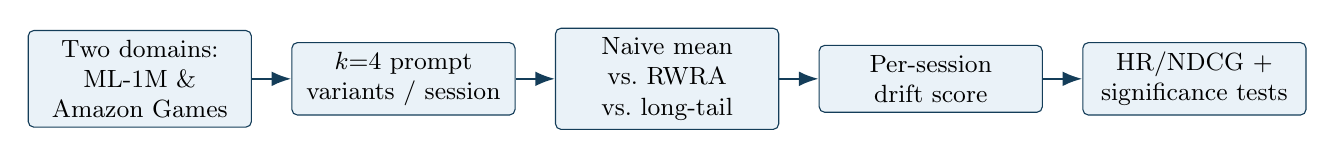
\begin{tikzpicture}[
  node distance=0.5cm,
  every node/.style={font=\small},
  stage/.style={draw=DeepBlue, rounded corners=2pt, fill=SoftBlue,
               minimum height=0.85cm, text width=2.6cm, align=center},
  arrow/.style={-{Latex[length=2.5mm]}, thick, DeepBlue}
]
\node[stage] (data) {Two domains:\\ML-1M \& Amazon Games};
\node[stage, right=of data] (ens) {$k{=}4$ prompt\\variants / session};
\node[stage, right=of ens] (agg) {Naive mean\\vs.\ RWRA\\vs.\ long-tail};
\node[stage, right=of agg] (drift) {Per-session\\drift score};
\node[stage, right=of drift] (eval) {HR/NDCG +\\significance tests};
\draw[arrow] (data) -- (ens);
\draw[arrow] (ens) -- (agg);
\draw[arrow] (agg) -- (drift);
\draw[arrow] (drift) -- (eval);
\end{tikzpicture}}

\vspace{0.6em}
\begin{block}{Design principle}
Every condition -- single prompt, naive ensemble, Reliability-Weighted Rank
Aggregation (RWRA), and long-tail-weighted RWRA -- is evaluated on the
\emph{same} sessions and candidate pools; only the aggregation strategy
changes.
\end{block}
\end{frame}

% ============================================================ Frame 13
\begin{frame}{Methodology -- dataset and experimental design}
\begin{table}
\centering
\small
\begin{tabular}{lrr}
\toprule
\textbf{Property} & \textbf{MovieLens-1M} & \textbf{Amazon Games}\\
\midrule
Sessions (leave-one-out) & 6{,}040 & 94{,}762\\
Candidate pool size & 20 & 20\\
Negative sampling & training-only popularity & training-only popularity\\
Domain noun in prompt & ``movie'' & ``game''\\
\bottomrule
\end{tabular}
\end{table}

\begin{itemize}
  \item Chronological leave-one-out: last interaction per user is the
        hidden target; everything before it is the visible prefix.
  \item Target is excluded from the prefix and never revealed as ``the
        answer'' -- prevents leakage.
  \item Amazon reviewer IDs / ASINs remapped to dense integer IDs so the
        rest of the pipeline is dataset-agnostic.
  \item For tractable local-LLM runtime, ensemble evaluation uses a
        matched, seeded random sample (equal size per domain), not the
        full 94{,}762-session Amazon set.
\end{itemize}
\end{frame}

% ============================================================ Frame 14  [NEW]
\begin{frame}{Methodology -- output protocol and strict parsing}
\begin{block}{The output contract}
The model returns one numeric score in the range 0--100 for every
candidate \emph{position}:
\vspace{0.3em}
\centerline{\code{\{"scores": [85, 42, 91, \ldots]\}}}
\end{block}

\vspace{0.5em}
\begin{itemize}
  \item Ranking is performed by the \emph{program} (descending score, ties
        broken by position), not by the model. The model never emits item
        IDs, so numerals inside titles (``Xbox 360'') cannot be mistaken
        for ranking positions.
  \item Responses violating the schema are recorded as \emph{parsing
        failures} together with the raw text -- never silently repaired,
        since repairing them would hide the unreliability being measured.
  \item A parsing failure (output unusable) is counted separately from a
        recommendation failure (valid output, target ranked low).
\end{itemize}
\end{frame}

% ============================================================ Frame 15
\begin{frame}{Methodology -- RWRA Step 1: ensemble scoring}
\begin{block}{The idea}
Instead of trusting a single prompt's ranking, \emph{Reliability-Weighted
Rank Aggregation} (RWRA) scores every candidate under several controlled
prompt variants of the \emph{same} model, then combines the results.
\end{block}

\vspace{0.7em}
\begin{itemize}
  \item For each session, score the 20-item candidate pool under $k{=}4$
        wording variants of the baseline prompt.
  \item Same session, same candidates, same model, same decoding settings
        (temperature 0, top-p 1) -- only the wording instruction changes.
  \item This is the same local model run four times, not four different
        models -- no extra training, no extra model to maintain.
\end{itemize}
\end{frame}

% ============================================================ Frame 16
\begin{frame}{Methodology -- RWRA Step 2: per-trial reliability weight}
\begin{block}{Definition}
Each member's weight is its mean Kendall's $\tau$ rank-agreement with
every other member, shifted to be non-negative and normalized to sum to 1:
\end{block}

\vspace{0.8em}
\[
w_i \;=\; \frac{\tau_i + 1}{\sum_j (\tau_j + 1)}, \qquad
\tau_i = \frac{1}{k-1}\sum_{j \neq i} \mathrm{KendallTau}(r_i, r_j)
\]

\vspace{0.8em}
\begin{itemize}
  \item $\tau_i \in [-1, 1]$; the $+1$ shift guarantees every weight is
        non-negative before normalizing.
  \item No labeled calibration data is needed -- the weight comes purely
        from how much this trial's members agree with each other.
\end{itemize}
\end{frame}

% ============================================================ Frame 17
\begin{frame}{Methodology -- RWRA Step 3: aggregation}
\begin{block}{Final score}
\[
\text{score} \;=\; \sum_i w_i \cdot \text{score}_i
\]
\end{block}

\vspace{0.8em}
\begin{exampleblock}{What this achieves}
A member whose ranking disagrees with the rest of the ensemble for
\emph{this specific session} is automatically downweighted -- a variant
that happens to be an outlier only for this session, not in general, stops
distorting the result without ever being manually flagged.
\end{exampleblock}
\end{frame}

% ============================================================ Frame 18  [NEW]
\begin{frame}{Methodology -- per-session drift score}
\begin{block}{Definition}
The same pairwise agreement computation that produces the weights also
yields a diagnostic: the mean Kendall's $\tau$ over all member pairs for
this session, reported alongside mean Jaccard@5 and Jaccard@10 overlap.
\end{block}

\vspace{0.7em}
\[
\text{drift}_s \;=\; \frac{2}{k(k-1)}\sum_{i<j} \mathrm{KendallTau}(r_i, r_j)
\]

\vspace{0.7em}
\begin{itemize}
  \item Near $+1$: all prompt variants agreed -- the model was stable here.
  \item Low or negative: the ensemble split -- the model was unstable on
        this session, and its recommendation deserves caution.
\end{itemize}

\vspace{0.4em}
\centering
\textcolor{DeepBlue}{One statistic, two uses: the weights \emph{and} the diagnostic.}
\end{frame}

% ============================================================ Frame 19
\begin{frame}{Methodology -- long-tail weighting: the adaptation}
\begin{alertblock}{Adapted from Llama4Rec}
Llama4Rec blends an LLM and a \emph{separately trained conventional
recommender}, weighted by how sparse a \emph{user's} interaction history
is.
\end{alertblock}

\vspace{0.8em}
\begin{block}{The substitution made here}
This work has only one model family (the LLM), so the same mechanism is
repurposed: it blends the \textbf{RWRA ensemble} with the \textbf{single
baseline prompt}, weighted by how short \emph{this session's prefix} is --
not by a separately trained model's confidence.
\end{block}

\vspace{0.5em}
\centering
\textcolor{DeepBlue}{\emph{Two models, weighted by user sparsity}
$\;\longrightarrow\;$
\emph{One model, ensembled and weighted by session sparsity.}}
\end{frame}

% ============================================================ Frame 20
\begin{frame}{Methodology -- long-tail weighting: formulas}
\[
\ell_s = \log(\text{prefix\_length}+1)
\]
\[
\beta_s = \max\!\left(\frac{\ell_{\max}-\ell_s}{\ell_{\max}-\ell_{\min}},\,\beta_2\right)\cdot\beta_1
\]
\[
\text{score}_s \;=\; \beta_s \cdot \text{RWRA}_s \;+\; (1-\beta_s)\cdot \text{baseline}_s
\]

\vspace{0.5em}
\begin{itemize}
  \item Short-prefix (``cold'') sessions $\Rightarrow$ higher $\beta_s$
        $\Rightarrow$ trust the ensemble more.
  \item Long-prefix (``warm'') sessions $\Rightarrow$ lower $\beta_s$
        $\Rightarrow$ a single prompt may already be reliable enough.
  \item $\ell_{\min}, \ell_{\max}$ are computed once over the full dataset,
        so a session's weight is stable regardless of which subsample is
        evaluated.
\end{itemize}
\end{frame}

% ============================================================ Frame 21
\begin{frame}{Evaluation protocol}
\begin{columns}[T]
\column{0.48\linewidth}
\textbf{Accuracy metrics}
\begin{itemize}
  \item HR@1, HR@5, HR@10
  \item NDCG@5, NDCG@10
  \item Computed identically for all 4 conditions via one shared module.
\end{itemize}

\textbf{Stability metrics}
\begin{itemize}
  \item Mean pairwise Kendall's $\tau$ across ensemble members.
  \item Mean pairwise Jaccard@5 / Jaccard@10.
\end{itemize}

\column{0.48\linewidth}
\textbf{Statistical testing}
\begin{itemize}
  \item Paired bootstrap confidence interval (2000 resamples) on
        reciprocal rank, per pairwise comparison.
  \item Paired Wilcoxon signed-rank test.
  \item Comparisons restricted to sessions valid under \emph{both}
        compared conditions.
\end{itemize}

\textbf{Stratified analysis}
\begin{itemize}
  \item All 4 conditions recomputed on short / medium / long
        prefix-length tertiles -- directly tests RQ3.
\end{itemize}
\end{columns}
\end{frame}

% ============================================================ Frame 22
\begin{frame}{Implementation status}
\begin{block}{What is built and unit-tested (honest status)}
\begin{itemize}
  \item Full data pipeline for both domains; RWRA and long-tail-weighted
        aggregation; statistical testing module.
  \item \textbf{75 automated tests, all passing} -- including tests that
        verify RWRA correctly downweights a synthetically divergent
        ensemble member.
  \item End-to-end pipeline verified with a deterministic stub model
        (no network/GPU needed) on both domains.
\end{itemize}
\end{block}

\vspace{0.4em}
\begin{alertblock}{What is \emph{not} yet done -- stated plainly}
Real-LLM evaluation at scale has not been run yet. The only real-model
evidence so far is a small pilot (next slide); full-scale runs are the
immediate next step, pending accelerated compute access.
\end{alertblock}
\end{frame}

% ============================================================ Frame 23
\begin{frame}{Preliminary pilot evidence -- not final results}
\begin{table}
\centering
\small
\begin{tabular}{lrrrrr}
\toprule
\textbf{Wording variant} & \textbf{HR@1} & \textbf{HR@5} & \textbf{HR@10} & \textbf{NDCG@5} & \textbf{NDCG@10}\\
\midrule
baseline\_scores\_v1 & 0.20 & 0.20 & 0.40 & 0.200 & 0.263\\
wording\_direct\_v1 & 0.40 & 0.40 & 0.60 & 0.400 & 0.460\\
\bottomrule
\end{tabular}
\end{table}

\vspace{0.5em}
\begin{alertblock}{How to read this table}
$n{=}5$ sessions per condition. This was run to confirm the model produces
parseable output under each wording variant -- it is a \emph{pipeline
validation}, far too small for any statistical claim. It is shown only as
evidence that the sensitivity under investigation is present.
\end{alertblock}
\source{Qwen2.5-3B-Instruct via Ollama, temperature 0, top-p 1, deterministic decoding.}
\end{frame}

% ============================================================ Frame 24
\begin{frame}{Conclusion I -- contribution}
\begin{block}{Targeted contribution}
\begin{itemize}
  \item A reliability-weighting method for LLM session recommenders that
        needs no frontier model and no second trained model.
  \item A per-session drift metric operationalizing ``semantic drift''
        as an inspectable number, not just an accuracy drop.
  \item A long-tail-aware extension, honestly adapted from Llama4Rec's
        mechanism to a single-model setting.
  \item Cross-domain evaluation (movies and games) with no domain-specific
        tuning.
\end{itemize}
\end{block}
\end{frame}

% ============================================================ Frame 25
\begin{frame}{Conclusion II -- next steps}
\begin{block}{Immediate next steps}
\begin{enumerate}
  \item Small real-model validation run (both domains).
  \item Full sampled-scale run with real statistics.
  \item Stratified long-tail analysis on real results.
  \item Final write-up with honest limitations.
\end{enumerate}
\end{block}

\vspace{1em}
\centering
\Large\textcolor{DeepBlue}{Same small model. More evidence, weighted by how much it agrees with itself.}
\end{frame}

\end{document}
